\apendice{Documentación técnica de programación}

\section{Introducción}
En este apartado se mostrarán los distintos requisitos e instrucciones necesarias para la instalación y comprensión del proyecto. Para ello se deberá tener en cuenta:
\begin{enumerate}
    \item \textbf{Estructura de directorios}: se mostrará la estructura general del proyecto. Este apartado también se puede observar en el repositorio de  \textit{GitHub} que contendrá, a parte de la estructura de directorios, las tareas realizadas. 
    \item \textbf{Manual del programador}: manual en el que se exponen los pasos a seguir para poder continuar con el proyecto. 
    \item \textbf{Compilación, instalación y ejecución del proyecto}: manual que abarca las instrucciones básicas para poder ejecutar el proyecto.  
    \item \textbf{Pruebas del sistema}, explicación de las distintas pruebas realizadas y de como lanzarlas.
\end{enumerate}

\section{Estructura de directorios}
En este subapartado se comentará la estructura del contenido del proyecto. Es la misma que la que se puede apreciar en el repositorio de \texttt{\textit{GitHub}}\footnote{https://github.com/lnc1002/TFG-Evaluacion-Ejercicios-Rehabilitacion.git}:

\dirtree{%
.1 /.
.2 app.
.3 VideosCompletos\_Ej\_OFF.
.3 VideosCompletos\_Ej\_ON.
.3 VideosConcretos\_Ej\_OFF.
.3 VideosConcretos\_Ej\_ON.
.2 doc.
.3 Vídeos.
.3 Látex.
.4 img.
.4 tex.
.2 src.
.3 dockers.
.4 fishubu.
.5 base.
.5 enviroment.
.4 kafka.
.4 spark.
.5 base.
.5 master.
.5 worker.
.3 process.
.4 model.
.4 testvideos.
.3 prueba.
.3 pruebas.
.4 Pickle.
.4 vídeos.
.4 img.
.3 scripts.
.4 deploy.
.4 helpers.
.3 tools.
.4 jupyter.
.4 videos.
.5 processed.
.5 raw.
.2 README.md.
.2 LICENSE.
.2 gitignore.
}

Como se puede observar, de la raíz cuelgan las carpetas \texttt{app, src, doc} y tres documentos con las siguientes funcionalidades:
\begin{enumerate}
    \item \texttt{README.md}: documento que se encuentra en la raíz del repositorio de \textit{GitHub} y aparecerá en más directorios. Este fichero muestra información relativa al proyecto y a los ficheros que contiene el directorio en el que se ubica. Está compuesto por un resumen y unas instrucciones básicas de como está estructurado el contenido del proyecto.
    \item \texttt{LICENSE}: documento que contiene la licencia del proyecto en \textit{GitHub}.
    \item \texttt{.gitignore}: documento que especifica que archivos o directorios no se desean subir al repositorio. 
\end{enumerate}

\subsection{Documentación}
Una vez comentada la estructura de ficheros se va a exponer la estructura de los directorios que cuelgan desde la raíz del proyecto. La carpeta \texttt{doc} contiene toda la documentación del proyecto y tiene la siguiente estructura:
\dirtree{%
.1 doc.
.2 Latex.
.3 img.
.3 tex.
.2 Videos.
.2 Readme.md.
}

Dentro del directorio \texttt{Latex} se encuentra toda la documentación de memoria y anexos realizada sobre \LaTeX. En la carpeta \texttt{/doc/Latex/img} se localizan todas las imágenes y diagramas usados en este proyecto. Tanto una gran cantidad de imágenes como de diagramas han sido realizados con la herramienta \textit{Diagrams.net} \cite{wiki:drawio}. 

En el directorio \texttt{Videos} se encuentran unos breves vídeos del funcionamiento de como ejecutar el proyecto, obtener los \textit{frames} resultantes a partir de los \textit{pickle} generados y como interactuar con la aplicación de escritorio. 

\newpage
\subsection{Código}
La carpeta \texttt{src} contiene todos los ficheros y directorios necesarios tanto para ejecutar el programa como para la localización de las secuencias. En concreto vamos a exponer el contenido del directorio \texttt{/src/scripts/deploy/}:
\dirtree{%
.1 src.
.2 scripts.
.3 deploy.
.4 new-stream.
.4 start-server.
.4 stop-server.
.4 stop-stream.
.4 classify\_exercises.py.
.4 find\_frames.py.
}

Los dos últimos ficheros son los que se han implementado para poder localizar la secuencia o clasificar el ejercicio una vez haya terminado el proceso de extracción de posiciones.

Por otra parte, el directorio \texttt{/src/pruebas/} contiene:
\dirtree{%
.1 src.
.2 pruebas.
.3 C1\_Pruebas\_paquetes\_DTW.ipynb.
.3 C2\_Buscar\_Subsecuencia.ipynb.
.3 C3\_Busqueda\_y\_agrupacion\_de\_secuencia\_SIMILAR.ipynb.
.3 C4\_Busqueda\_multiples\_secuencias.ipynb.
.3 C5\_Busqueda\_inicio\_y\_final.ipynb.
.3 C6\_Pruebas\_busqueda\_angulos.ipynb.
.3 C7\_Pruebas\_busqueda\_posiciones.ipynb.
.3 C8\_Pruebas\_recortando\_frames.ipynb.
.3 C9\_Pruebas\_clasificacion\_movimientos.ipynb.
.3 C10\_Resultados\_finales.ipynb.
.3 Pickle.
.4 Posiciones\_inferiores.
.4 Posiciones\_superiores.
.4 Posiciones\_completas.
.4 Angulos\_completos.
.3 vídeos.
.3 img.
.3 README.md.
}

Como se puede observar dentro de este directorio se encuentran los diferentes \textit{notebooks} que se han empleado para mostrar las pruebas realizadas durante todo el proceso del proyecto. Además en el directorio \texttt{/src/pruebas/Pickle} se encuentran almacenadas gran parte de las secuencias generadas y en el directorio \texttt{/src/pruebas/vídeos} algunos de los vídeos creados para dichas pruebas. 


\subsection{Aplicación}
La carpeta \textbf{app} contiene todos los ficheros y directorios necesarios para poder ejecutar la aplicación de escritorio y su estructura es la siguiente:
\dirtree{%
.1 app.
.2 VideosCompletos\_Ej\_OFF.
.2 VideosCompletos\_Ej\_ON.
.2 VideosConcretos\_Ej\_OFF.
.2 VideosConcretos\_Ej\_ON.
.2 .gitignore.
.2 MiddleWindow.py.
.2 PredictWindow.py.
.2 main.py.
.2 README.md.
.2 requirements.txt.
}

\section{Manual del programador}

Todo el proyecto ha corrido sobre la máquina \textit{gamma} del equipo \textit{ADMIRABLE} de la Universidad de Burgos y para poder llevar a cabo las ejecuciones se han tenido que instalar una serie de programas sobre el entorno de \textit{Ubuntu}.
Muchos de estos programas han sido instalados mediante el comando \textit{wget} y el entorno final ha quedado con los siguientes programas y versiones:
\begin{enumerate}
    \item \textbf{Anaconda}: es una distribución de \textit{Python} utilizada para el desarrollo científico tanto gráfico como analítico \cite{wiki:anaconda}. En este proyecto se ha utilizado la versión \textbf{conda 4.11.0}.
    \item \textbf{NVIDIA}: es un \textit{software} que ofrece una amplia gama de posibilidades para la construcción o aceleración de aplicaciones \cite{wiki:nvidia}. En este proyecto se ha utilizado la versión \textbf{460.80}.
    \item \textbf{CUDA}: es una plataforma de computación paralela  y un modelo de programación desarrollados por \textit{NVIDIA} \cite{wiki:cuda}. En este proyecto se ha utilizado la versión de CUDA \textbf{ 11.2}.
    \item \textbf{Detectron2}: es una plataforma para la detección de objetos ~\cite{wu2019detectron2}.En este proyecto se ha utilizado la versión 0.6. Para más información sobre \textit{Detectron2} visitar el apartado de la memoria \textit{Técnicas y herramientas}.
    \item \textbf{Tensorflow}: es una plataforma de código abierto que cuenta con una amplia cantidad de herramientas y recursos para el aprendizaje automático \cite{wiki:tensorflow}. En este proyecto se ha utilizado la versión \textbf{2.8.0}.
\end{enumerate}


\subsection{\textit{Script} de despliegue}
\textcolor{blue}{Este apartado ha sido extraído del \textit{Script} de despliegue de José Luis Garrido Labrador}

Para el despliegue de los servicios mediante \textit{Docker} se han creado cuatro \textit{scripts} localizados en la carpeta \texttt{src/scripts/deploy}. Estos códigos en \textit{Bash} son los siguientes:
\begin{enumerate}
    \item \textbf{start-server}: se encarga de instanciar los diferentes servicios.
    \begin{lstlisting}[language=Bash]
 Sintaxis
	    start-server <Carpeta de salida> <N. de CPU master> <N. de workers> <N. de CPU por worker> <Memoria por worker>
    \end{lstlisting}
    \item \textbf{stop-server}: detiene todos los servicios.
    \begin{lstlisting}[language=Bash]
 Sintaxis
	    stop-server
    \end{lstlisting}
    \item \textbf{new-stream}: \label{cap:newstream} genera un nuevo flujo completo que se va a procesar. El funcionamiento es transparente. Recibe los parámetros para el \texttt{emitter.py} y para el \texttt{consumer.py}. Por seguridad es preferible solamente modificar los parámetros de gestión del flujo y no los de comunicación. Devuelve el identificador del flujo. Es importante este valor para poder cerrarlo después.
    \begin{lstlisting}[language=Bash]
 Sintaxis
    	new-stream "Parámetros emitter.py" "Parámetros consumer.py"
    	# Es muy importante mantener las comillas
    \end{lstlisting}
    \item \textbf{stop-stream}: detiene todos los procesos sobre un flujo concreto.
    \begin{lstlisting}[language=Bash]
 Sintaxis
	    stop-stream <ID del flujo>
    \end{lstlisting}
\end{enumerate}


\subsection{\textit{Script} de análisis}
Para la comparación de secuencias se han creado dos \textit{scripts}:
\begin{enumerate}
    \item \textbf{find\_frames.py}: localiza el patrón de referencia dentro de la secuencia de mayor tamaño y devolverá los \textit{frames} en los que se ha iniciado y finalizado la supuesta secuencia encontrada. Por último devolverá también una clasificación del tipo de ejercicio realizado.
    \begin{lstlisting}[language=Bash]
 Sintaxis
	    find_frames.py <secuencia del ejercicio concreto> <secuencia con varios ejercicios>
    \end{lstlisting}
    \item \textbf{classify\_exercises.py}: informará del tipo de ejercicio que se está realizando en el vídeo pasado como argumento.
    \begin{lstlisting}[language=Bash]
 Sintaxis
	    classify_exercises.py <secuencia del ejercicio concreto> 
    \end{lstlisting}
\end{enumerate}

\newpage
\section{Compilación, instalación y ejecución del proyecto}
\textcolor{blue}{Parte de este apartado ha sido extraído del apartado de \textit{Compilación, instalación y ejecución del proyecto} de José Luis Garrido Labrador}

Como se ha mencionado anteriormente, en la carpeta \texttt{src/scripts/deploy} se encuentran los \textit{scripts} para instalar el proyecto y poder ejecutarlo.

Para que los \textit{scripts} se ejecuten correctamente es necesario que se corran sobre un sistema operativo GNU/Linux con el servicio \textit{Docker} y la extensión \textit{Nvidia container toolkit} ~\cite{toolkitnvidiadocker} instalados. Adicionalmente se necesitará que la máquina donde se vayan a ejecutar los \textit{workers} disponga de una tarjeta gráfica \textit{Nvidia} instalada con soporte para \textit{CUDA} 10.2. 

Es posible que sea necesario cambiar el fichero \textit{Dockerfile} de la \texttt{carpeta dockers/fishubu/base} para que use los drivers de la tarjeta gráfica del equipo sobre el que se lanza la imagen \textit{docker}.


Antes de lanzar los servicios es importante haber creado previamente las imágenes maestras \textbf{(orden build)} para los diferentes \textit{dockers}. Desde la carpeta deploy:
\begin{lstlisting}[language=Bash]
docker build -f ../../dockers/fishubu/base/Dockerfile -t fishubu-base:1.0.0 ../../
docker build -f ../../dockers/fishubu/enviroment/Dockerfile -t fishubu-env:1.0.0 ../../
docker build ../../dockers/spark/base -t spark-base-fis:2.4.5
docker build ../../dockers/spark/master -t spark-master-fis:2.4.5
docker build ../../dockers/spark/worker -t spark-worker-fis:2.4.5
\end{lstlisting}

El orden de ejecución de los \textit{scripts} es el siguiente:

\begin{enumerate}
	\item \textbf{Ejecutar \texttt{start-server}} para que los servicios de \textit{Kafka} y \textit{Spark} estén activos y den soporte a los flujos que lo necesiten.
	\item \textbf{Ejecutar \texttt{new-stream}} recibiendo como parámetros la configuración deseada para el emisor y para el consumidor.  Este devuelve el identificador del flujo, será necesario para pedir el cierre del flujo.
\end{enumerate}

Para detener el flujo los pasos son los siguientes:
\begin{enumerate}
	\item \textbf{Ejecutar \texttt{stop-stream}} para cada flujo arrancado.
	\item \textbf{Ejecutar \texttt{stop-server}} y se detendrán todos los servicios.
\end{enumerate}

Para localizar la secuencia y clasificar los ejercicios el orden en el que se realicen las ejecuciones es indiferente. Por otra parte, tampoco es necesario que se esté corriendo el programa que extrae las secuencias, simplemente se necesitará tener algunas de ellas almacenadas:
\begin{enumerate}
    \item \textbf{Ejecutar \texttt{find\_frames.py}} para la extracción de la secuencia.
    \item \textbf{Ejecutar \texttt{classify\_exercises.py}} para la clasificación del ejercicio.
\end{enumerate}

\section{Fallos y soluciones} \label{cap:FallosSoluciones}
En este apartado se van a exponer algunos de los errores por los que se ha visto comprometido el proyecto, sus causas y sus posibles soluciones. 

Los fallos que producidos durante el trascurso de las ejecuciones son almacenados en diferentes ficheros. Por una parte se encuentran los ficheros de \textit{\textbf{log}} ubicados en el directorio \texttt{/tmp/fishubulogs}. Para consultar estos ficheros será necesario indicar el identificador correspondiente al flujo lanzado, de esta forma los comandos a ejecutar serían los siguientes:
\begin{enumerate}
    \item Consultar el fichero \textit{\textbf{log-error}}:
    \begin{lstlisting}[language=Bash]
 Sintaxis
	    cd /tmp/fishubulogs/log-error-{id-stream} 
    \end{lstlisting}
    \item Consultar el fichero \textit{\textbf{log}}:
    \begin{lstlisting}[language=Bash]
 Sintaxis
	    cd /tmp/fishubulogs/log-{id-stream} 
    \end{lstlisting}
\end{enumerate}

Otros errores serán almacenados en la carpeta \textit{\textbf{logs}} de cada máquina \textit{docker} ejecutada. Para poder observar estos errores será necesario adentrarse en el contender del que se quiera obtener información, esta acción se realiza mediante alguno de los siguientes comandos:
\begin{lstlisting}[language=Bash]
 Sintaxis
	    docker exec -it <container_name> bash}
\end{lstlisting}
\begin{lstlisting}[language=Bash]
 Sintaxis
	    docker exec -it <container_id> bash}
\end{lstlisting}

\subsection{Fallos de memoria}
\subsubsection{Fallos en la caída del flujo}
\textcolor{blue}{Parte del fallo redactado por Jose Luis Garrido Labrador y ampliado por Lucía Núñez Calvo}

Si la caída del flujo deja una excepción del tipo \textit{\textbf{Caused by: java.io.EOFException}}, como se puede observar en la figura \ref{f:EOFException}, o se observa el siguiente mensaje de error dentro del \textit{script} {/tmp/fishubulogs/log-error-{id-stream}} \textit{\textbf{StreamingContext: StreamingContext has already been stopped}} como se puede apreciar en la figura \ref{f:StreamingContext}, implica que los datos que debe procesar el flujo son mayores que los que caben en memoria.
Para solucionar este problema será necesario dar más memoria a cada \textit{worker}. El valor recomendado es de 2 GiB por cada núcleo de \textit{worker} pero se puede aumentar si el usuario lo considera oportuno.

\begin{figure}[H]
 \centering
\subfloat{
    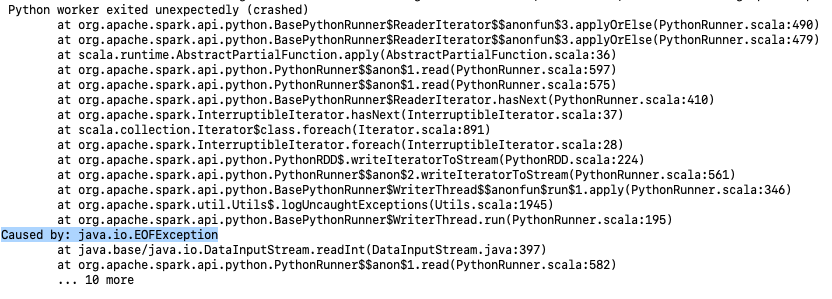
\includegraphics[width=\textwidth]{plantillaLatex-master/img/EOFException.png}}
 \caption{Error de tipo \textit{Caused by: java.io.EOFException}.}
 \label{f:EOFException}
\end{figure}

\begin{figure}[H]
 \centering
\subfloat{
    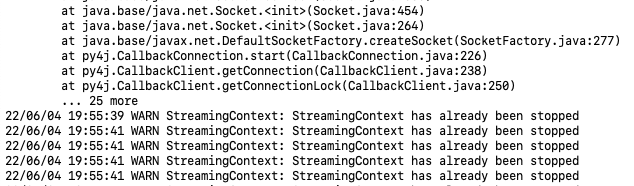
\includegraphics[width=\textwidth]{plantillaLatex-master/img/StreamingContext.png}}
 \caption{Error de tipo \textit{StreamingContext: StreamingContext has already been stop-ped}.}
 \label{f:StreamingContext}
\end{figure}


\subsubsection{Fallos con \textit{Docker}}

En caso de que se proceda al lanzamiento de los contenedores y la salida por pantalla sea \textit{\textbf{The server is not running}}, como se observa en la figura \ref{f:servernotrunning}, el problema puede ser que se haya agotado la memoria en el directorio \texttt{/var/cache/apt/archives/}. Para solventar este problema se tendrá que ejecutar siguiente el comando:
\begin{lstlisting}[language=Bash]
 Sintaxis
	    docker system prune --all
\end{lstlisting}

Tras su ejecución se deberán restaurar las imágenes (orden build).

\begin{figure}[H]
 \centering
\subfloat{
    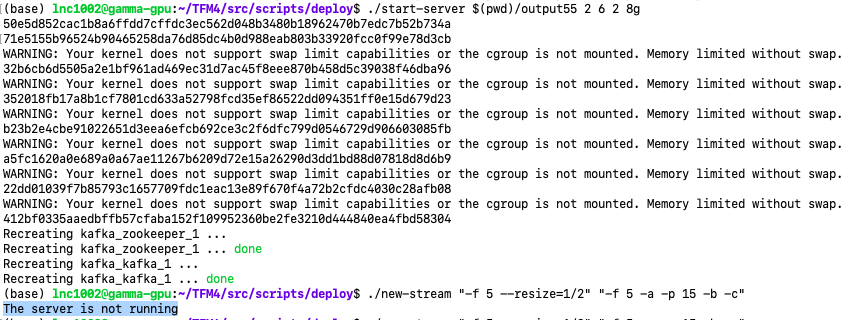
\includegraphics[width=\textwidth]{plantillaLatex-master/img/ServerNot.png}}
 \caption{Error de tipo \textit{The server is not running}.}
 \label{f:servernotrunning}
\end{figure}

\subsection{Error de permisos}
Si el proyecto se está ejecutando sobre la máquina \textit{gamma} del grupo \textit{ADMIRABLE} de la Universidad de Burgos y tras intentar lanzar el servidor aparecen numerosos mensajes de tipo \textit{\textbf{Get permission denied while trying to connect to the Docker daemon socket at unix}}, como el que se puede apreciar en la imagen \ref{f:permissionDe}, quiere decir que el usuario no está presente en el grupo \textit{docker}.

\begin{figure}[H]
 \centering
\subfloat{
    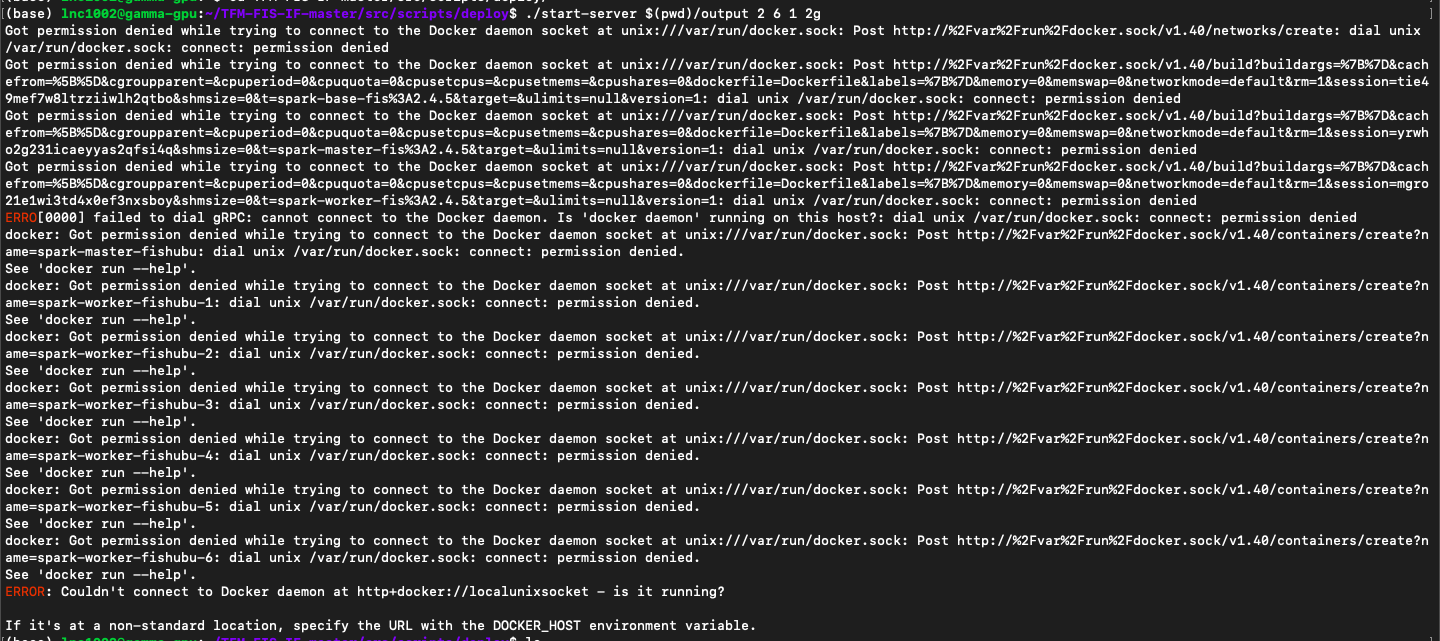
\includegraphics[width=\textwidth]{plantillaLatex-master/img/permissionDenied.png}}
 \caption{Error de tipo \textit{Get permission denied while trying to connect to the Docker daemon socket at unix}.}
 \label{f:permissionDe}
\end{figure}

Para solventar este problema, un administrador del sistema deberá ejecutar el siguiente comando:
\begin{lstlisting}[language=Bash]
 Sintaxis
	    usermod -a -G docker nombre-usuario
\end{lstlisting}

\subsection{Los fotogramas no se procesan}
\textcolor{blue}{Parte del fallo redactado por Jose Luis Garrido Labrador y ampliado por Lucía Núñez Calvo}

Si los fotogramas no se procesan y observa la existencia del fichero de \texttt{log/notprocesslog} en los \textit{workers}, significa que ha existido un error mientras se procesaba el fotograma. En el mismo \textit{\textbf{log}} se encuentra el origen del fallo y probablemente se deberá a que el fichero de \texttt{extraOpt.py} incluye información errónea o una ruta incorrecta.

Para solucionar esto se debe volver a cargar el fichero \texttt{extraOpt.py} y por tanto se han de volver a construir  las imágenes \emph{(orden build)} desde la \texttt{fishubu-env}. En el caso de que el error persista, usar el flag \emph{--no-cache} a
la hora de reconstruir las imágenes.

\subsection{Error de \textit{Kafka}}

Algunos de los errores que pueden aparecer ante un usuario impaciente son los siguiente, como se puede apreciar en la imagen \ref{f:kafkaerror}: 
\begin{enumerate}
    \item \textit{Error while executing topic command : Replication factor: 1 larger than available brokers: 0.
ERROR org.apache.kafka.common.errors.
InvalidReplicationFactorException: Replication factor: 1 larger than available brokers: 0. (kafka.admin.TopicCommand)}
    \item \textit{WARN [AdminClient clientId=adminclient-1] Connection to node -1 (localhost/127.0.0.1:9092) could not be established. Broker may not be available. (org.apache.kafka.clients.NetworkClient)}
\end{enumerate}

\begin{figure}[H]
 \centering
\subfloat{
    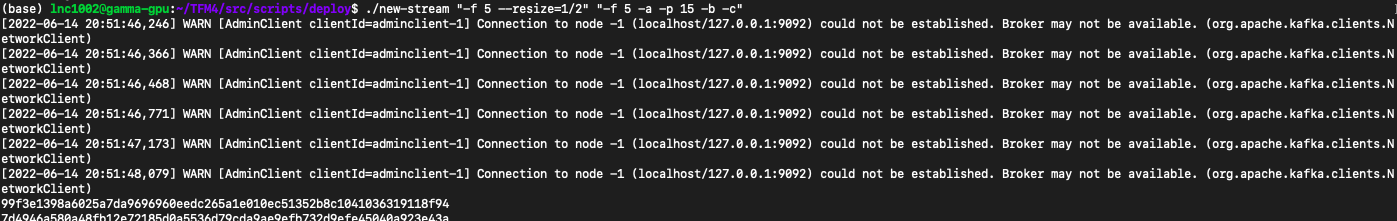
\includegraphics[width=\textwidth]{plantillaLatex-master/img/errorKafka.png}}
 \caption{Error de tipo \textit{kafka}.}
 \label{f:kafkaerror}
\end{figure}

Estos errores únicamente le informan al usuario de que no ha dejado suficiente tiempo para que se cargue \textit{Kafka} correctamente. El tiempo de carga puede variar por múltiples factores, por esa razón puede, que tras lanzar el servidor se intente crear un flujo y no nos muestre el error, mientras que en otras ocasiones si lo haga. Por ello, es recomendable dejar trascurrir unos segundos desde que se lanza el servidor. 

En caso de que aparezca este error, únicamente se pararía el flujo creado y se volverían a lanzar los contenedores. 


\subsection{Errores de versión de \textit{Nvidia}}
\textcolor{blue}{Redactado por Jose Luis Garrido Labrador}

Si a la hora de ejecutar el flujo, en el arranque ocurre una excepción del tipo \textit{\textbf{forward compatibility was attempted}} indica que la versión instalada de \textit{Nvidia} sobre \textit{docker} no es compatible con la versión instalada
en el equipo.

Para solucionarlo es necesario cambiar el fichero \emph{Dockerfile} de la carpeta \texttt{src/dockers/fishubu/base} y cambiar la versión que se instala por la que se tiene en el equipo. Es necesario que al menos sea la versión 440.

\subsection{Error con la conexión a \textit{Nvidia}}
\textcolor{blue}{Redactado por Jose Luis Garrido Labrador}

Si el flujo al iniciar da el error \textit{\textbf{could not select device driver}} significa que la extensión de \textit{docker} para la compatibilidad con \textit{Nvidia} no está instalada o no se ha reiniciado el servicio de \textit{docker} desde que se instaló.

Se soluciona instalando la extensión de \textit{docker «docker-nvidia»} y reiniciando el servicio.


\section{Pruebas del sistema}
Como se ha podido observar, el proyecto se ha dividido en dos fases principales. Una primera fase fue el análisis de librerías y la segunda fase fue condensar todo lo investigado en la implementación del objetivo del proyecto.

Prácticamente todas las pruebas se han corrido sobre distintos \textit{notebooks} ya que esta herramienta permite organizar de una manera muy intuitiva cómoda y visual los resultados obtenidos, pero ¿qué se entiende por pruebas?. 

Un aspecto a tener en cuenta es la dificultad de ejecutar pruebas unitarias en minería de datos. Para ejecutar una prueba se debe saber de manera previa el resultado, en nuestro caso este resultado sólo se consigue mediante un análisis visual por parte del usuario. Es el propio programador el que tiene que comprobar si la secuencia obtenidas se corresponde con la secuencia esperada. Este resultado se ha podido comprobar de dos maneras:
\begin{enumerate}
    \item \textbf{Pruebas mediante código}: el procedimiento a seguir para realizar este tipo de pruebas es muy sencillo. Tras analizar el vídeo que contiene la secuencia de ejercicios completos, localizamos visualmente el vídeo que queremos encontrar y nos quedamos con el instante de tiempo en el que comienza y finaliza. El siguiente paso es una mera regla de tres. Si se tienen un total de $X$ \textit{frames} y el vídeo cuenta con una duración de $Z$ instantes de tiempo, el momento justo en el que empieza o finaliza el ejercicio concreto encontrado dentro del vídeo que contiene todos los ejercicios será igual a
    \begin{equation}
        \frac{frame\_encontrado*Z}{X}
    \end{equation}
    \item \textbf{Pruebas mediante la aplicación de escritorio}: el procedimiento a realizar en este caso es más sencillo porque el cálculo anterior ya se encuentra implementado en la aplicación. En este caso será necesario cargar tanto el vídeo concreto como el vídeo que comprende toda la secuencia de ejercicios y proceder a recortar el vídeo. Visualizando el recorte en la aplicación se podrá comprobar lo bien o mal que se está detectando la secuencia.
\end{enumerate}

Finalmente comentar que las pruebas han sido esenciales en este proyecto para poder seleccionar el mejor algoritmo para el objetivo perseguido, es decir, el algoritmo que consiga localizar una amplia colección de secuencias en un tiempo relativamente aceptable. 


 
